\documentclass{beamer}

% Beamer style
%\usetheme[secheader]{Madrid}
\usetheme{CambridgeUS}
\usecolortheme[rgb={0.65,0.15,0.25}]{structure}
%\usefonttheme[onlymath]{serif}
\beamertemplatenavigationsymbolsempty
%\AtBeginSubsection

% Packages
%\usepackage[french]{babel}
\usepackage[latin1]{inputenc}
\usepackage{color}
\usepackage{dsfont, stmaryrd}
\usepackage{amsmath, amsfonts, amssymb}
\usepackage{stmaryrd}
\usepackage{epsfig}
\usepackage{/Latex/astats}
%\usepackage[all]{xy}
\usepackage{graphicx}

% Commands
\definecolor{darkred}{rgb}{0.65,0.15,0.25}
\newcommand{\emphase}[1]{\textcolor{darkred}{#1}}
\newcommand{\paragraph}[1]{\emphase{#1}}
\newcommand{\refer}[1]{\textcolor{blue}{\sl \cite{#1}}}
\newcommand{\Refer}[1]{\textcolor{blue}{\sl #1}}
\newcommand{\newblock}{}

% Symbols
\newcommand{\Abf}{{\bf A}}
\newcommand{\Beta}{\text{B}}
\newcommand{\betabf}{\mbox{\mathversion{bold}{$\beta$}}}
\newcommand{\Bcal}{\mathcal{B}}
\newcommand{\BIC}{\text{BIC}}
\newcommand{\dd}{\text{d}}
\newcommand{\Cbf}{{\bf C}}
\newcommand{\dbf}{{\bf d}}
\newcommand{\Dcal}{\mathcal{D}}
\newcommand{\Esp}{\mathbb{E}}
\newcommand{\Ebf}{{\bf E}}
\newcommand{\Ecal}{\mathcal{E}}
\newcommand{\Gcal}{\mathcal{G}}
\newcommand{\Gam}{\mathcal{G}\mbox{am}}
\newcommand{\Ibb}{\mathbb{I}}
\newcommand{\Ibf}{{\bf I}}
\newcommand{\ICL}{\text{ICL}}
\newcommand{\Cov}{\mathbb{C}\text{ov}}
\newcommand{\Corr}{\mathbb{C}\text{orr}}
\newcommand{\Var}{\mathbb{V}}
\newcommand{\Vsf}{\mathsf{V}}
\newcommand{\pen}{\text{pen}}
\newcommand{\Fcal}{\mathcal{F}}
\newcommand{\Hbf}{{\bf H}}
\newcommand{\Hcal}{\mathcal{H}}
\newcommand{\Jcal}{\mathcal{J}}
\newcommand{\Kbf}{{\bf K}}
\newcommand{\Lcal}{\mathcal{L}}
\newcommand{\Mcal}{\mathcal{M}}
\newcommand{\mbf}{{\bf m}}
\newcommand{\mum}{\mu(\mbf)}
\newcommand{\Ncal}{\mathcal{N}}
\newcommand{\Nbf}{{\bf N}}
\newcommand{\Nm}{N(\mbf)}
\newcommand{\Ocal}{\mathcal{O}}
\newcommand{\Obf}{{\bf 0}}
\newcommand{\Omegas}{\underset{s}{\Omega}}
\newcommand{\Pbf}{{\bf P}}
\newcommand{\Pcal}{\mathcal{P}}
\newcommand{\Qcal}{\mathcal{Q}}
\newcommand{\Rbb}{\mathbb{R}}
\newcommand{\Rcal}{\mathcal{R}}
\newcommand{\sbf}{{\bf s}}
\newcommand{\Sbf}{{\bf S}}
\newcommand{\Scal}{\mathcal{S}}
\newcommand{\Ucal}{\mathcal{U}}
\newcommand{\Vcal}{\mathcal{V}}
\newcommand{\Tbf}{{\bf T}}
\newcommand{\ubf}{{\bf u}}
\newcommand{\Ubf}{{\bf U}}
\newcommand{\Wbf}{{\bf W}}
\newcommand{\xbf}{{\bf x}}
\newcommand{\Xbf}{{\bf X}}
\newcommand{\Ybf}{{\bf Y}}
\newcommand{\Zbf}{{\bf Z}}
\newcommand{\pibf}{\mbox{\mathversion{bold}{$\pi$}}}
\newcommand{\Sigmabf}{\mbox{\mathversion{bold}{$\Sigma$}}}
\newcommand{\gammabf}{\mbox{\mathversion{bold}{$\gamma$}}}
\newcommand{\mubf}{\mbox{\mathversion{bold}{$\mu$}}}
\newcommand{\nubf}{\mbox{\mathversion{bold}{$\nu$}}}
\newcommand{\Thetabf}{\mbox{\mathversion{bold}{$\Theta$}}}
\newcommand{\thetabf}{\mbox{\mathversion{bold}{$\theta$}}}
\newcommand{\BP}{\text{BP}}
\newcommand{\EM}{\text{EM}}
\newcommand{\VEM}{\text{VEM}}
\newcommand{\VBEM}{\text{VB}}
\newcommand{\cst}{\text{cst}}
\newcommand{\obs}{\text{obs}}
\newcommand{\ra}{\emphase{$\rightarrow$~}}
\newcommand{\QZ}{Q_{\Zbf}}
\newcommand{\Qt}{Q_{\thetabf}}

% Directory
\newcommand{\fighd}{/RECHERCHE/RUPTURES/Exposes/Figures}

%--------------------------------------------------------------------
\title{Segmentation for CNV: A statistical view}

\author[UMR 518]{UMR 518: J. Aubert, E. Lebarbier, S. Robin}

\institute[AgroParisTech / INRA]{AgroParisTech / INRA \\
  \bigskip
  \begin{tabular}{ccccc}
    
\epsfig{file=/RECHERCHE/RESEAUX/Exposes/Figures/LogoINRA-Couleur.ps,
    width=2.5cm} & 
    \hspace{.5cm} &
    
\epsfig{file=/RECHERCHE/RESEAUX/Exposes/Figures/logagroptechsolo.eps,
    width=3.75cm} & 
    \hspace{.5cm} &
    \epsfig{file=/RECHERCHE/RESEAUX/Exposes/Figures/Logo-SSB.eps,
    width=2.5cm} \\ 
  \end{tabular} \\
  \bigskip
  }

\date[CNV-maize]{CNV-maize, kick-off meeting, November 2010, Clermont} 

%--------------------------------------------------------------------

%--------------------------------------------------------------------
%--------------------------------------------------------------------
\begin{document}
%--------------------------------------------------------------------
%--------------------------------------------------------------------

%--------------------------------------------------------------------
\frame{\titlepage
  }

%--------------------------------------------------------------------
%--------------------------------------------------------------------
\section{Segmentation: The basic problem}
%--------------------------------------------------------------------
\frame{\frametitle{Segmentation: The basic problem}

  %\vspace{-0.5cm}
  \begin{tabular}{cc}
    \begin{tabular}{p{.5\textwidth}}
      \paragraph{Data at hand:} for a given individual
      \begin{itemize}
      \item a sequence of \emphase{known positions} along the
        \emphase{reference genome}, labelled as
        $$
        t = 1, 2, \dots, n
        $$
      \item a signal measured \emphase{at each position}
        $$
        Y_t = \text{signal at position $t$}
        $$
      \end{itemize} \pause
    \end{tabular}
    &
    \begin{tabular}{p{.5\textwidth}}
      \hspace{-1cm}
      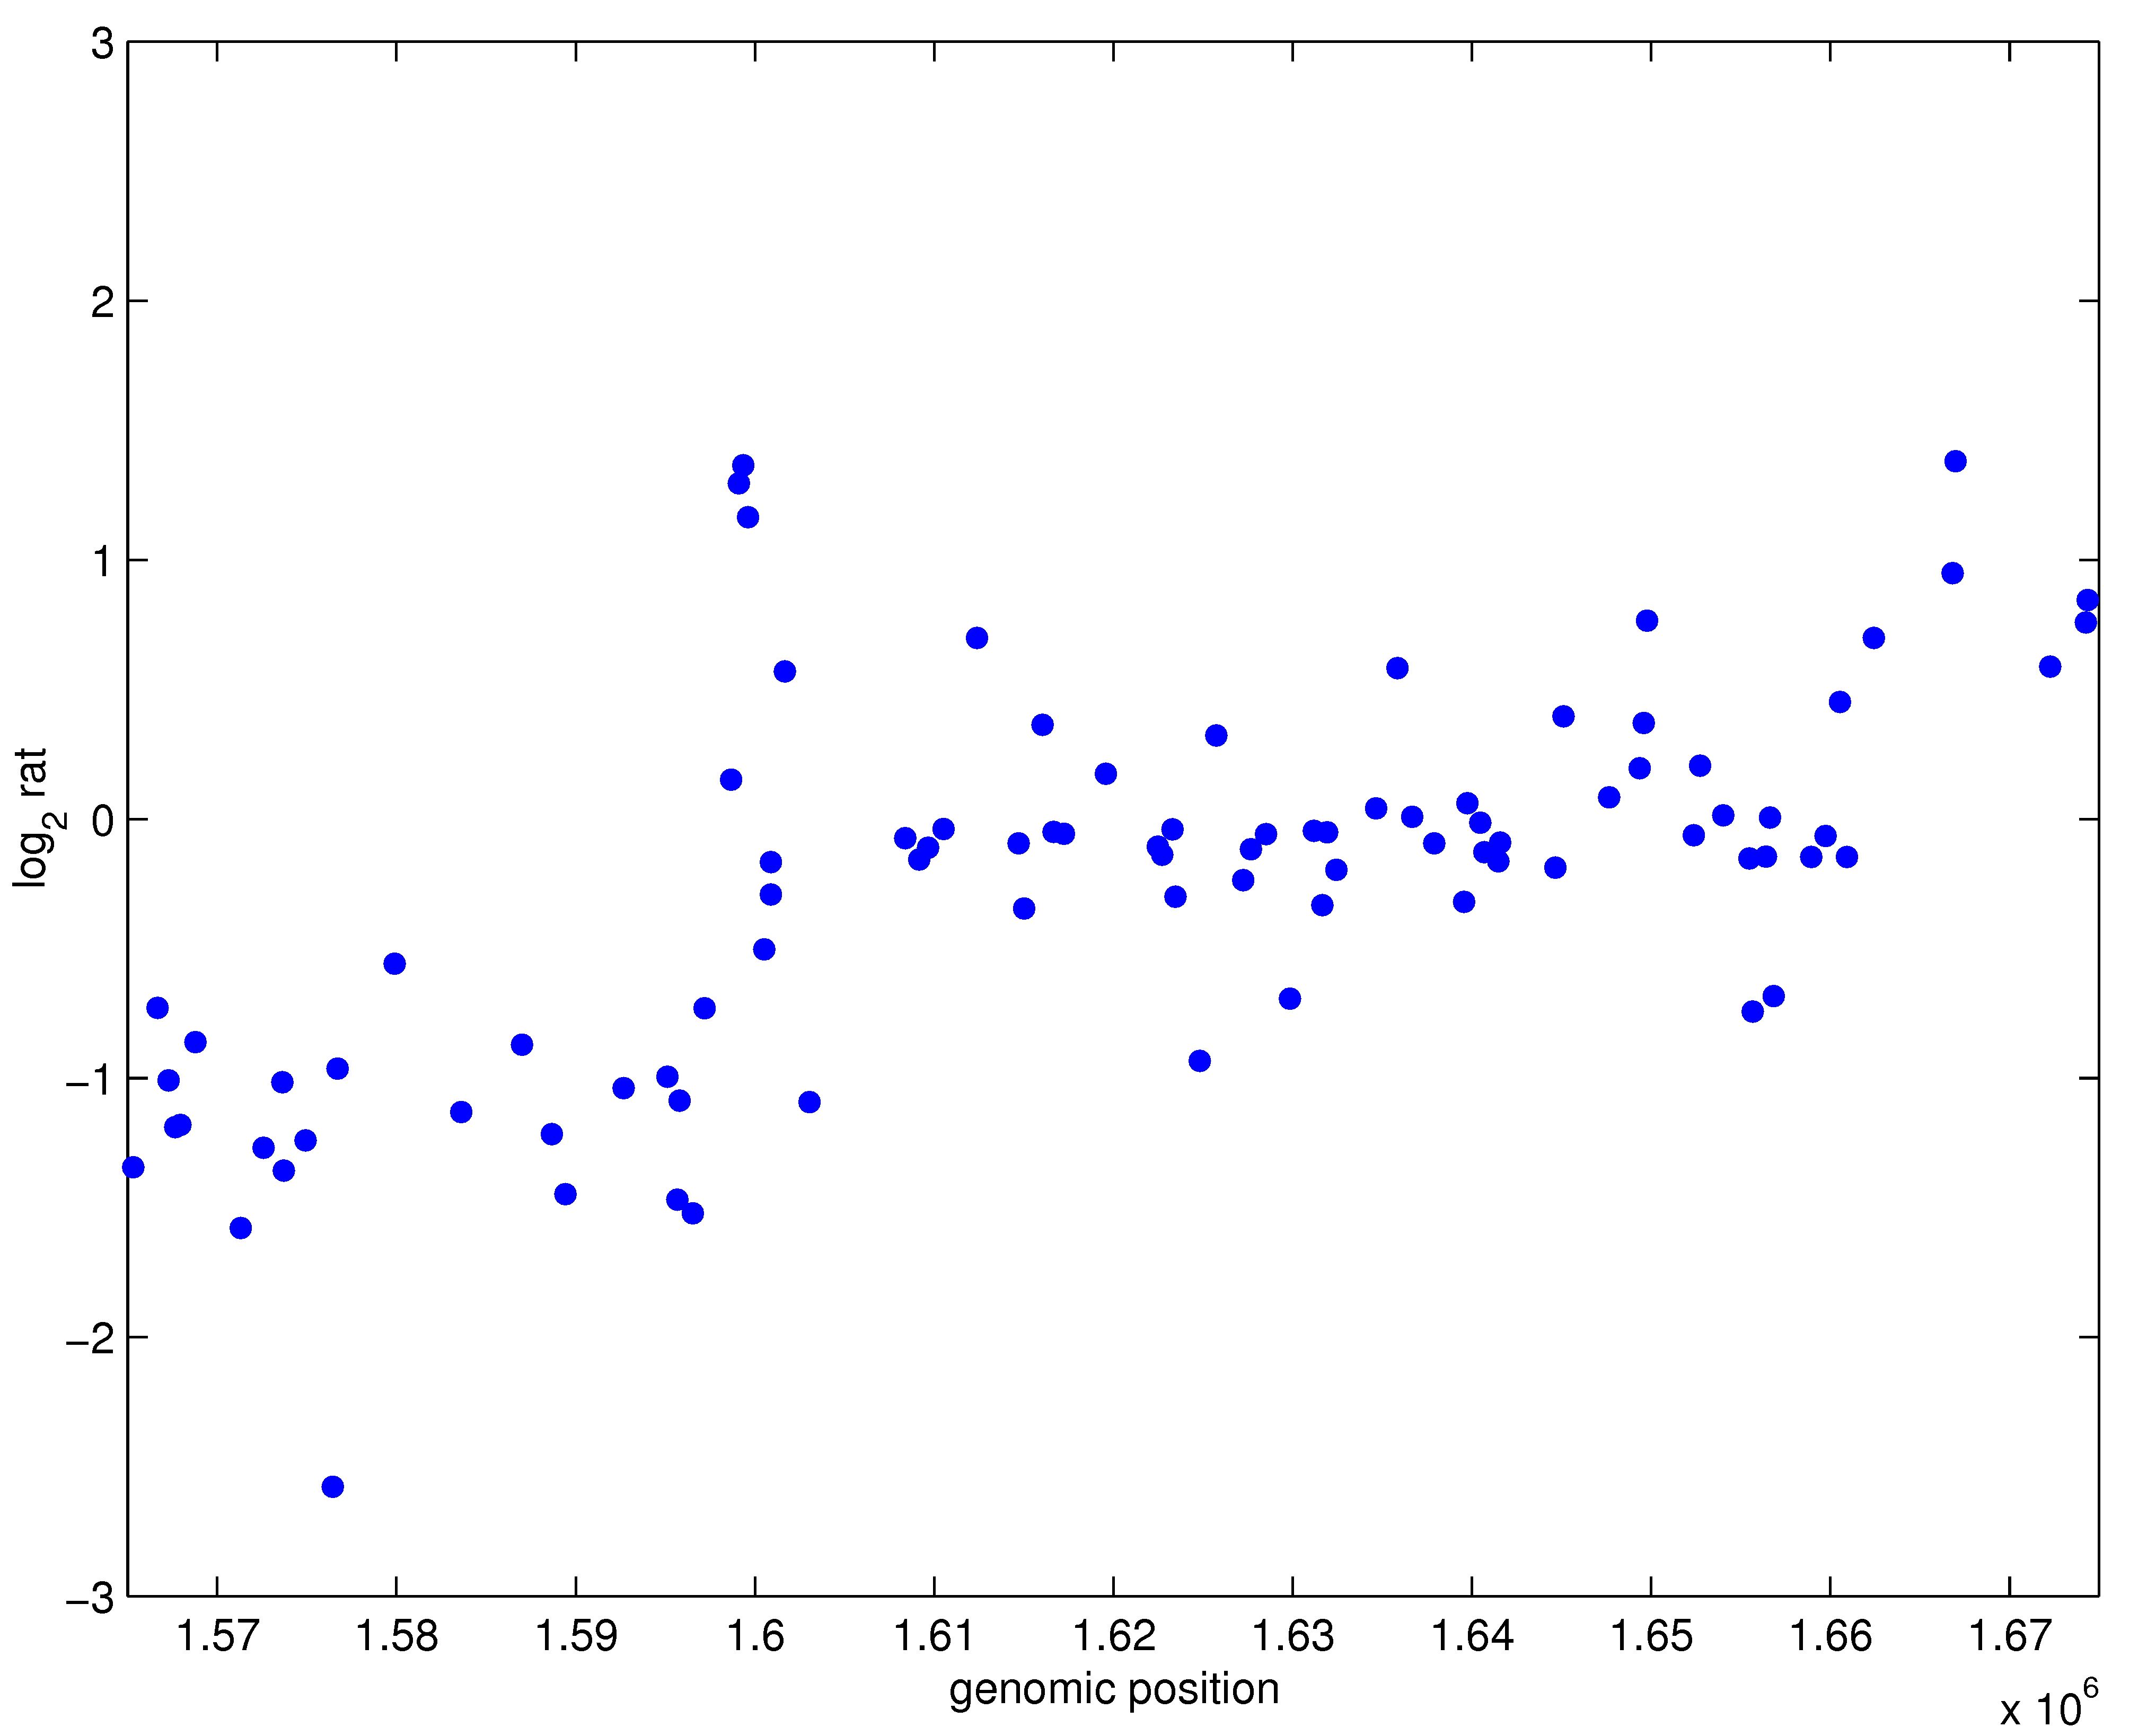
\epsfig{file = ../Figures/raw_profile_example.eps, clip=,
        width=.45\textwidth, height=.5\textheight}  
    \end{tabular}
  \end{tabular} \\
  \begin{eqnarray*}
    Y_t & \propto & f(\text{\emphase{relative copy number} at position }t) \\
    & = & \text{log-fluorescence, sum of the two allele signals for a given
      SNP, etc.}
  \end{eqnarray*}
  }

%--------------------------------------------------------------------
\frame{\frametitle{Segmentation: Basic model for a single profile}

  \paragraph{Basic model:} 
  \begin{itemize}
  \item \emphase{$\lambda_t = $ 'true' level} at position $t$ =
    f(relative copy number) \pause 
  \item the value of $\lambda_t$ is affected by \emphase{abrupt changes}:
    $$
    \epsfig{file = ../Figures/FigSeg_Intro.eps, clip=, bbllx=90,
      bblly=300, bburx=540, bbury=400, width=.7\textwidth} \pause
    $$
  \item the observed signal $Y_t$ is noisy:
    $$
    \mbox{for $t \in I_k$:} \qquad \emphase{Y_t = \mu_k + E_t}, \qquad
    \{E_t\} \text{ i.i.d. }  \sim \Ncal(0, \sigma^2). \pause
    $$
  \end{itemize}
  
  \paragraph{Aim:} infer the breakpoints positions
  \emphase{$\tau_1$, $\tau_2$, ...}, and the true level
  \emphase{$\mu_k$} in each segment \emphase{$I_k$} (and the noise
  variance \emphase{$\sigma^2$}).  
  
  }

%--------------------------------------------------------------------
\frame{\frametitle{To summarise}
  
  Modelling is supposed to help for the interpretation of the signal, \\
  that is to go from
  
  \bigskip
  \begin{tabular}{cc}
    \begin{tabular}{p{.5\textwidth}}
      \paragraph{there ...} \\
      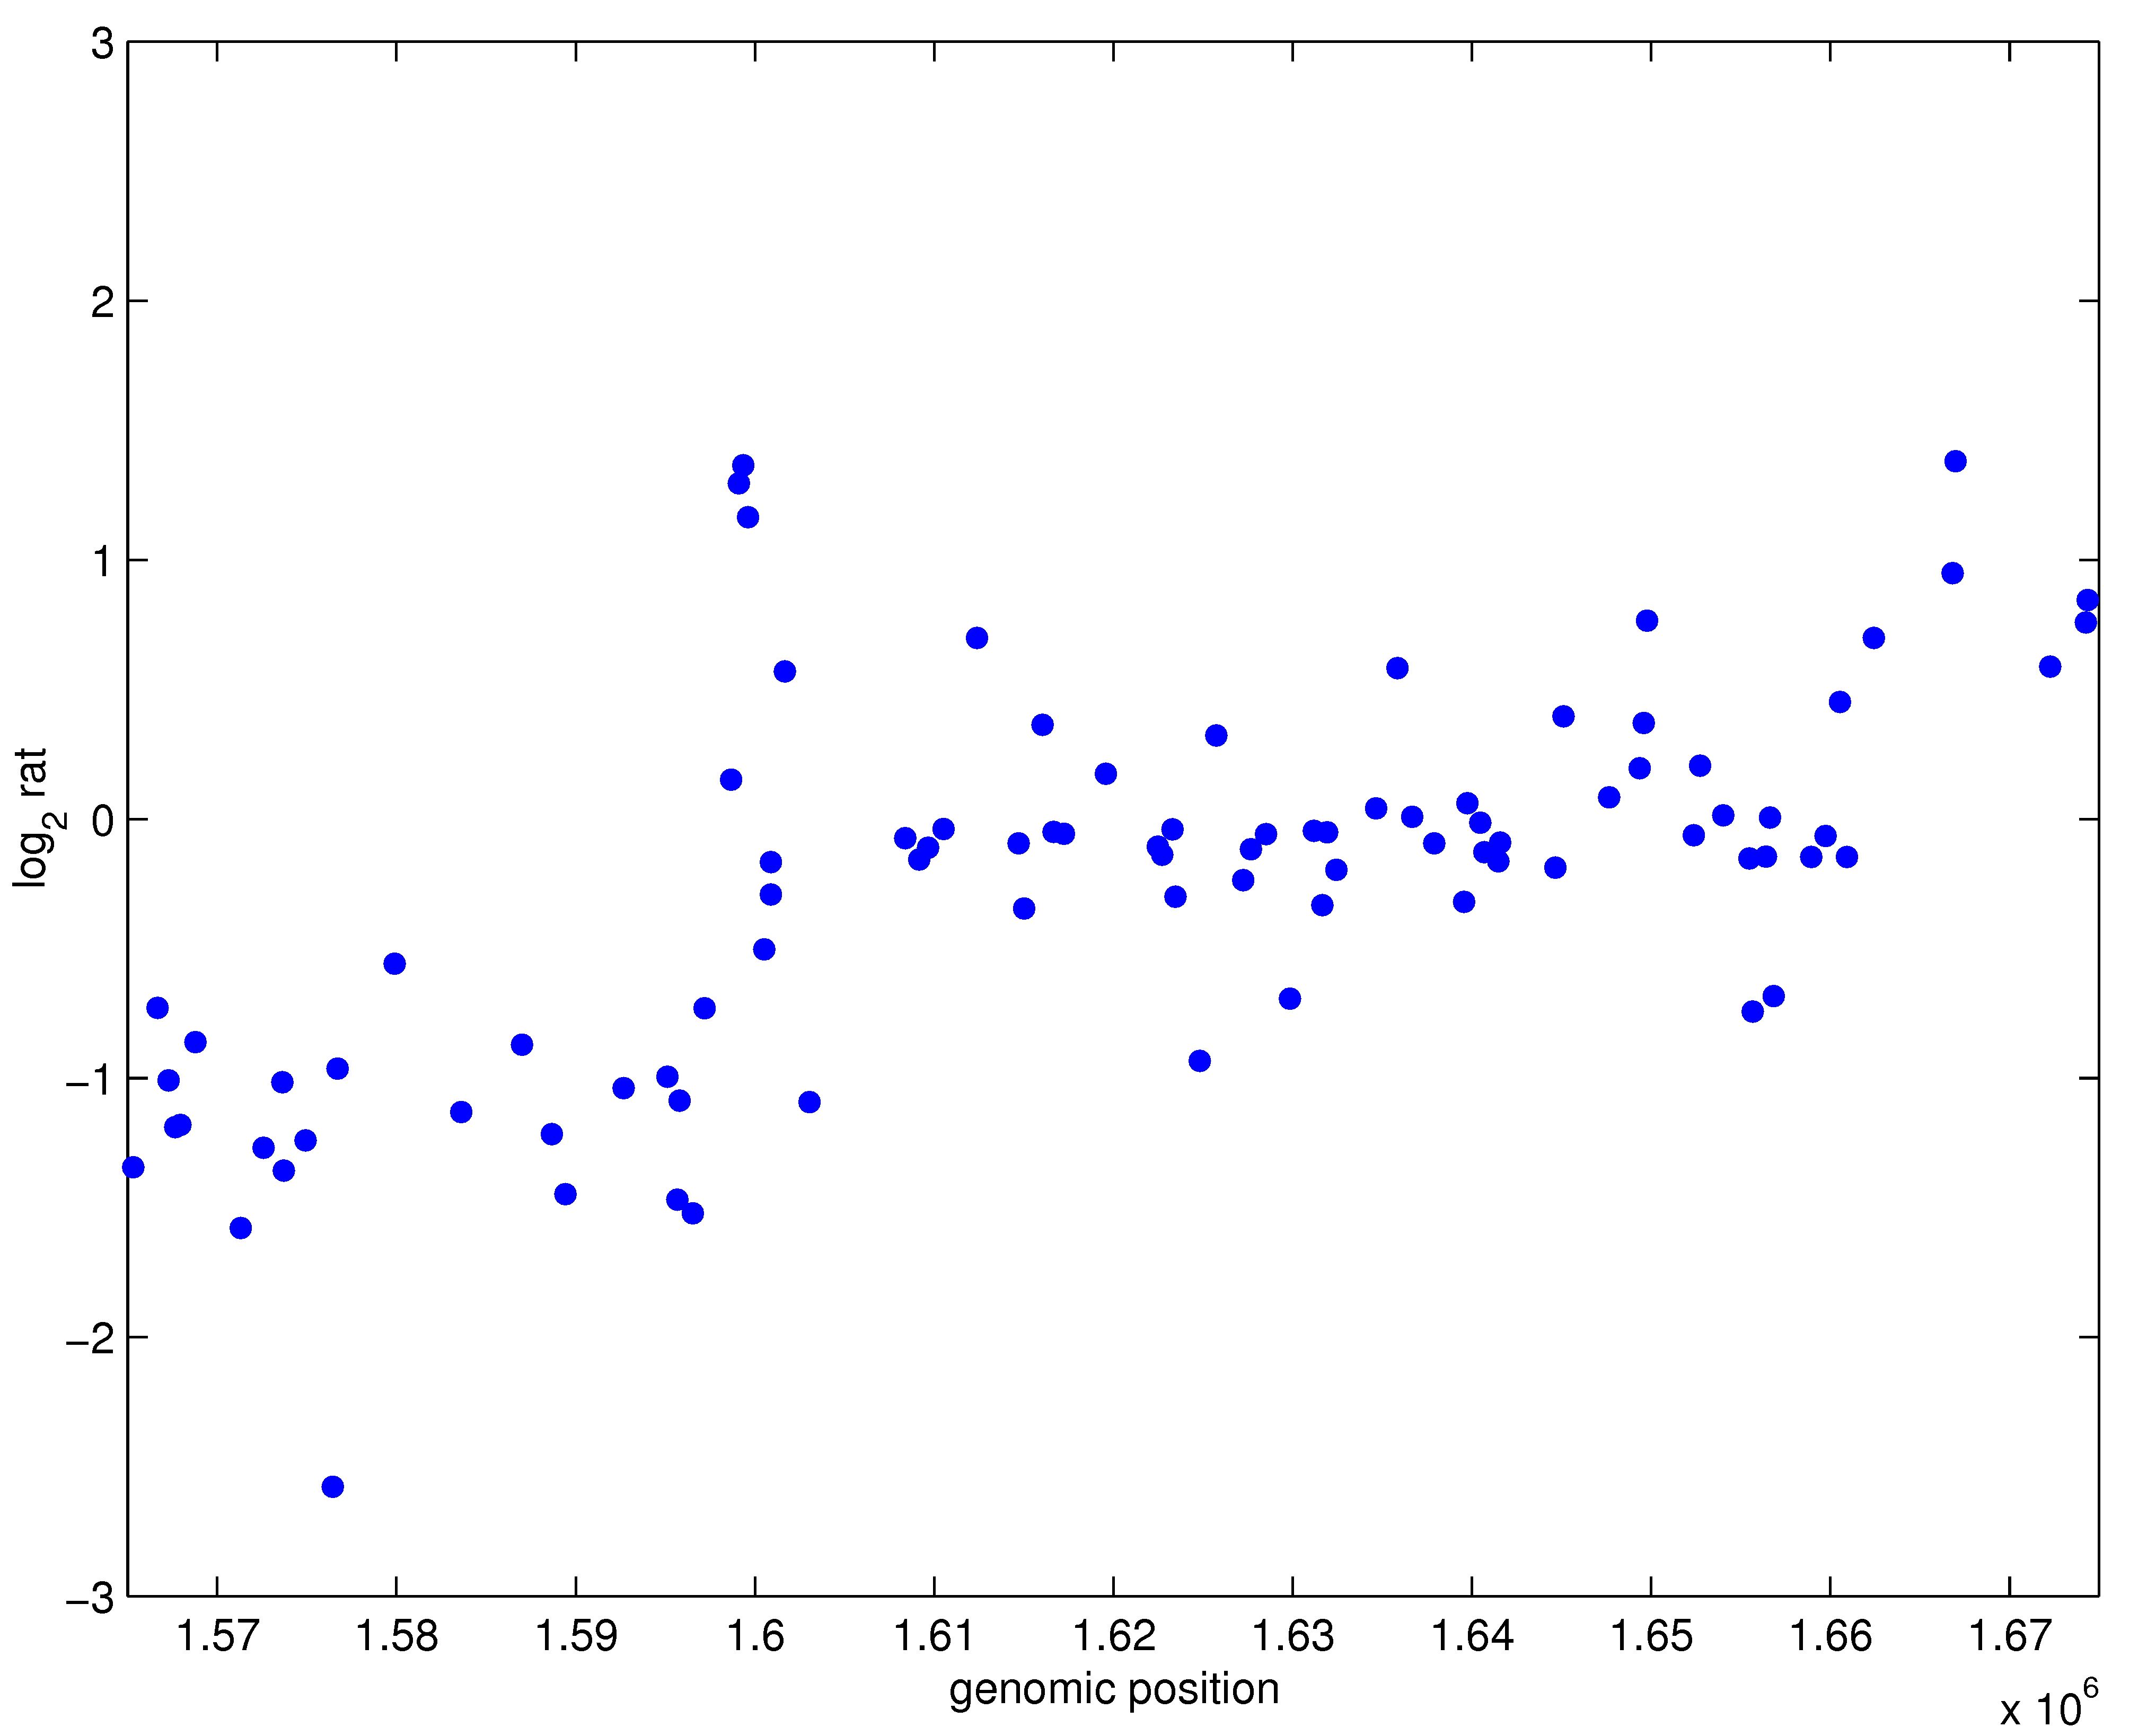
\epsfig{file = ../Figures/raw_profile_example.eps, clip=,
        width=.45\textwidth, height=.5\textheight}        
      \pause
    \end{tabular}
    &
    \hspace{-1cm}
    \begin{tabular}{p{.5\textwidth}}
      \paragraph{to there} \\
      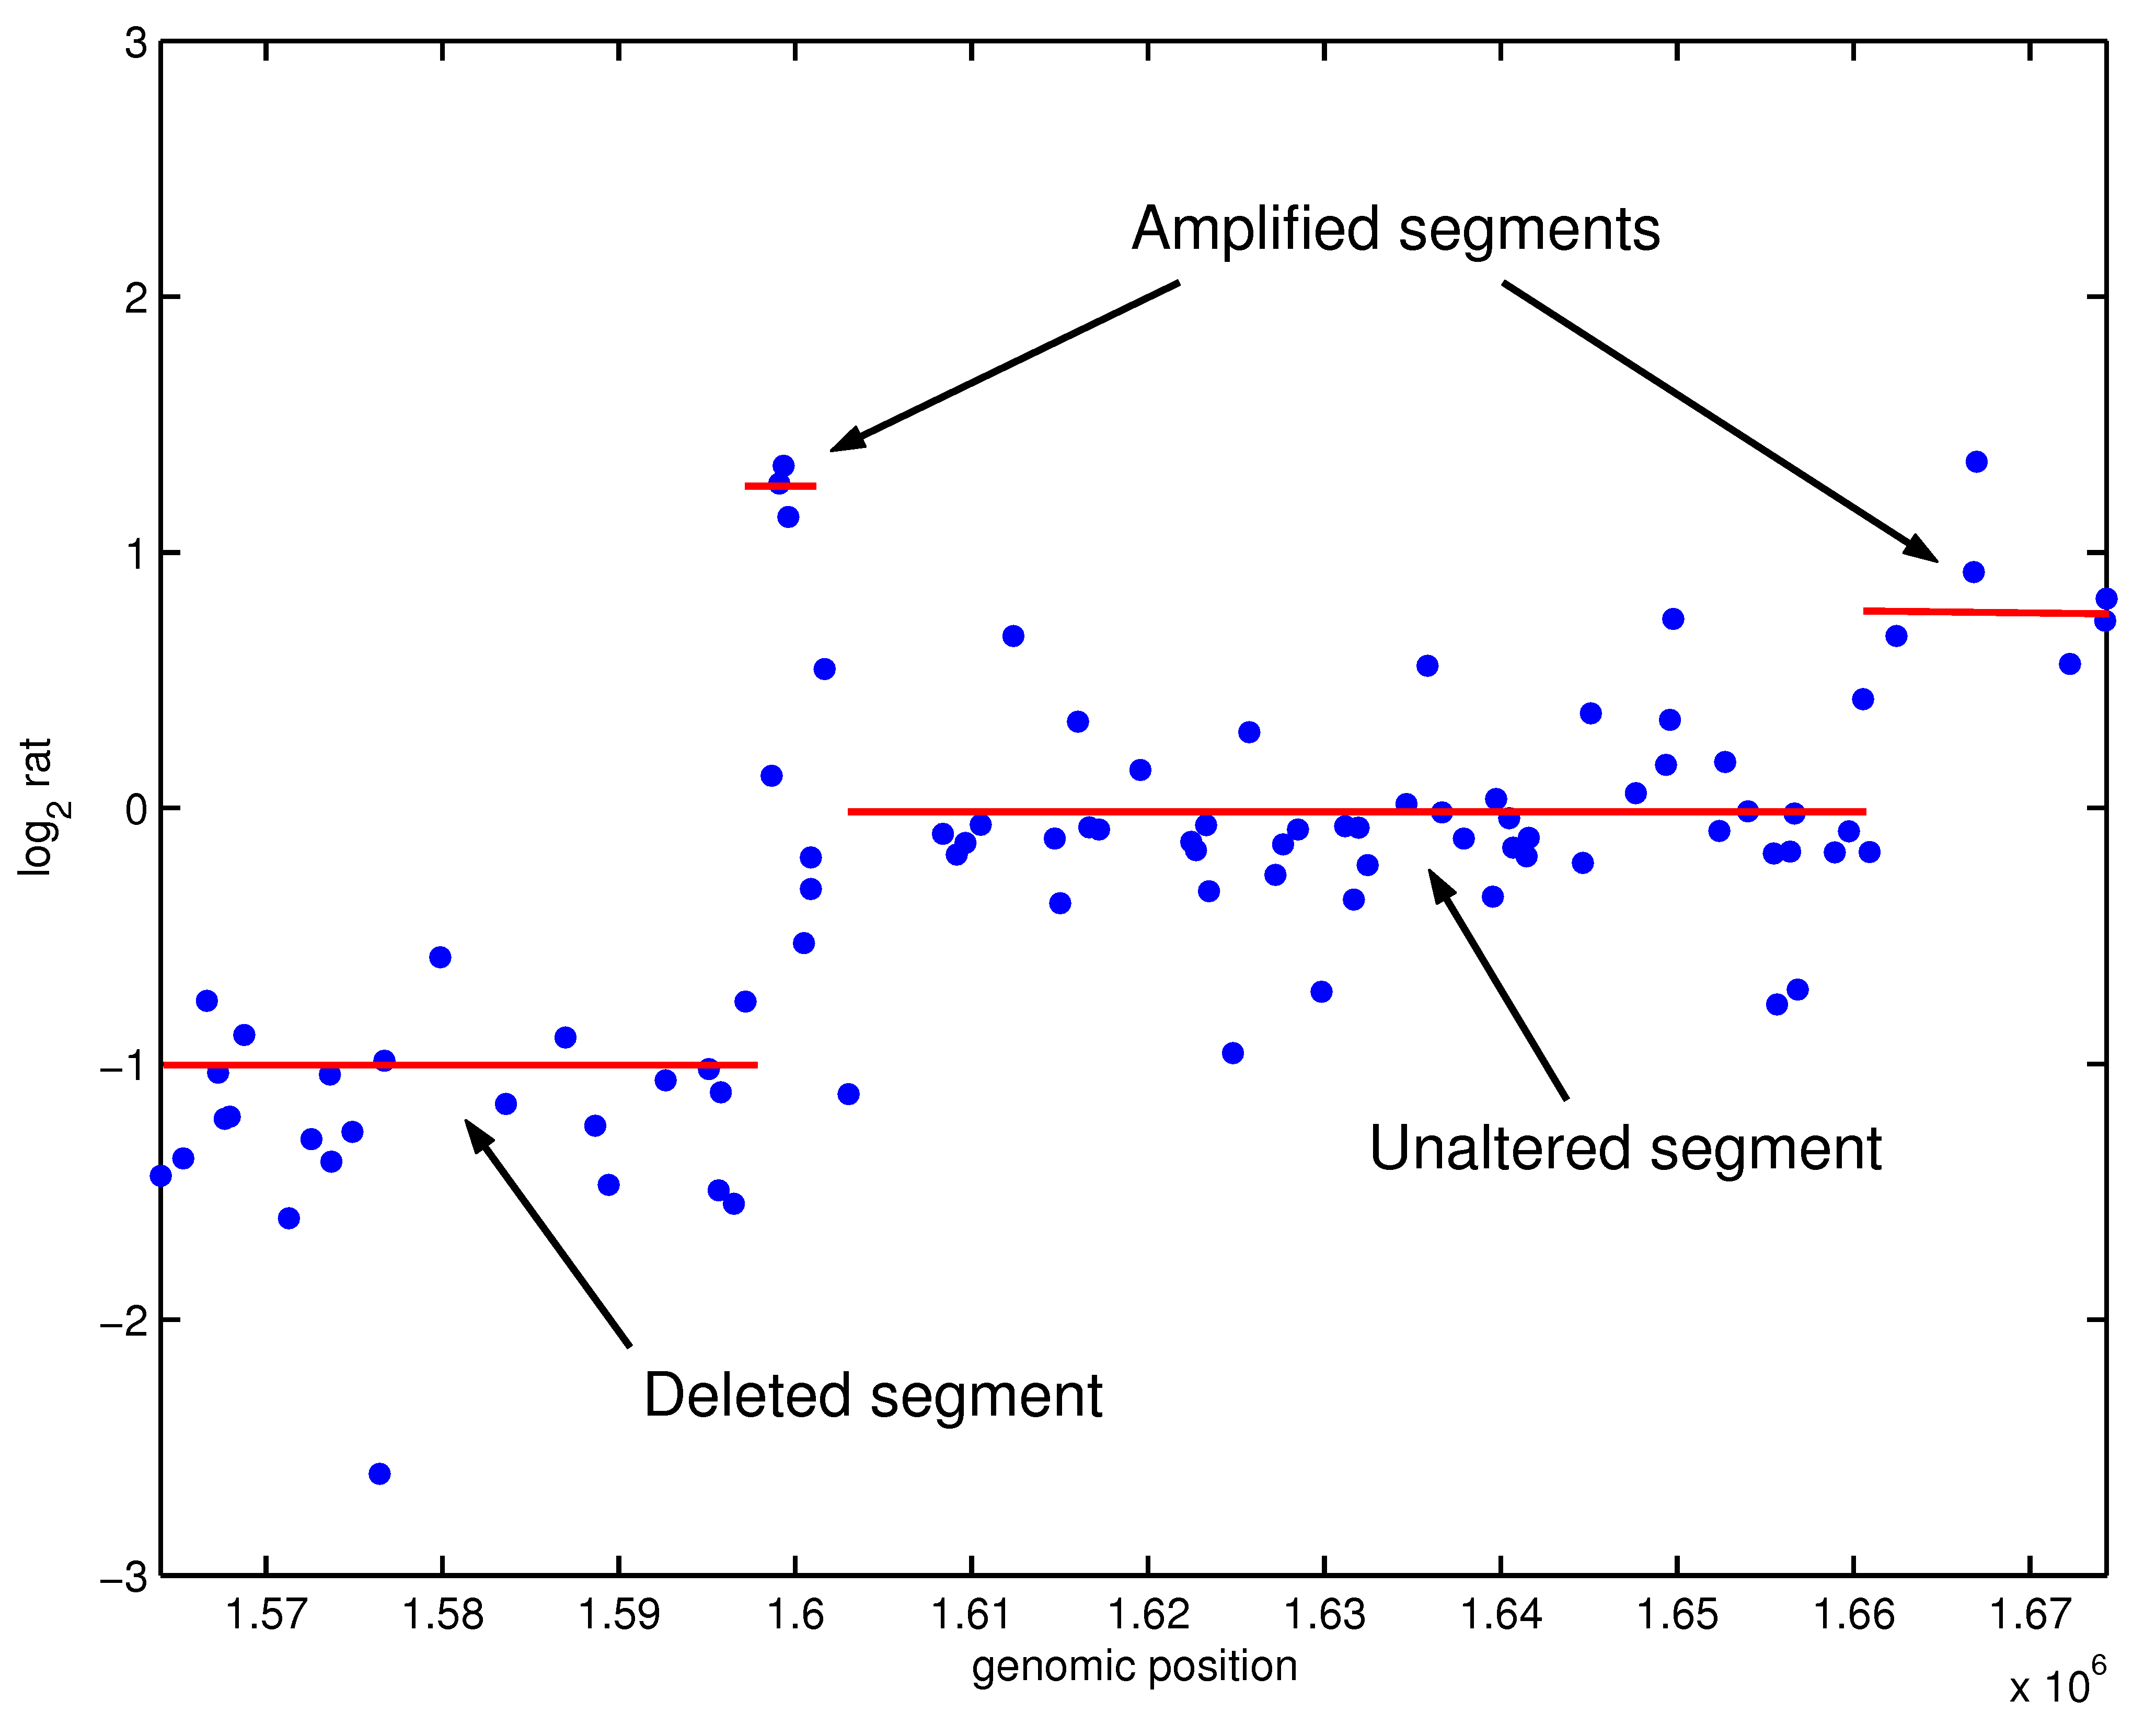
\epsfig{file = ../Figures/profile_example.eps, clip=,
        width=.45\textwidth, height=.5\textheight}  
    \end{tabular}
  \end{tabular}
  }

%--------------------------------------------------------------------
\subsection{Statistical inference}
%--------------------------------------------------------------------
\frame{\frametitle{Statistical inference}
  
  \emphase{For a given number $(K)$ of segments} estimates
  of $\tau_k$, $\mu_k$ derive from
  $$
  \min \sum_{k=1}^K \sum_{t \in \emphase{I_k}} (Y_t -
  \emphase{\mu_k})^2, \qquad I_k = \; ]\emphase{\tau_{k-1}};
  \emphase{\tau_k}]. \pause
  $$

  \begin{tabular}{cc}
    \hspace{-.5cm}
    \begin{tabular}{p{.5\textwidth}}
%       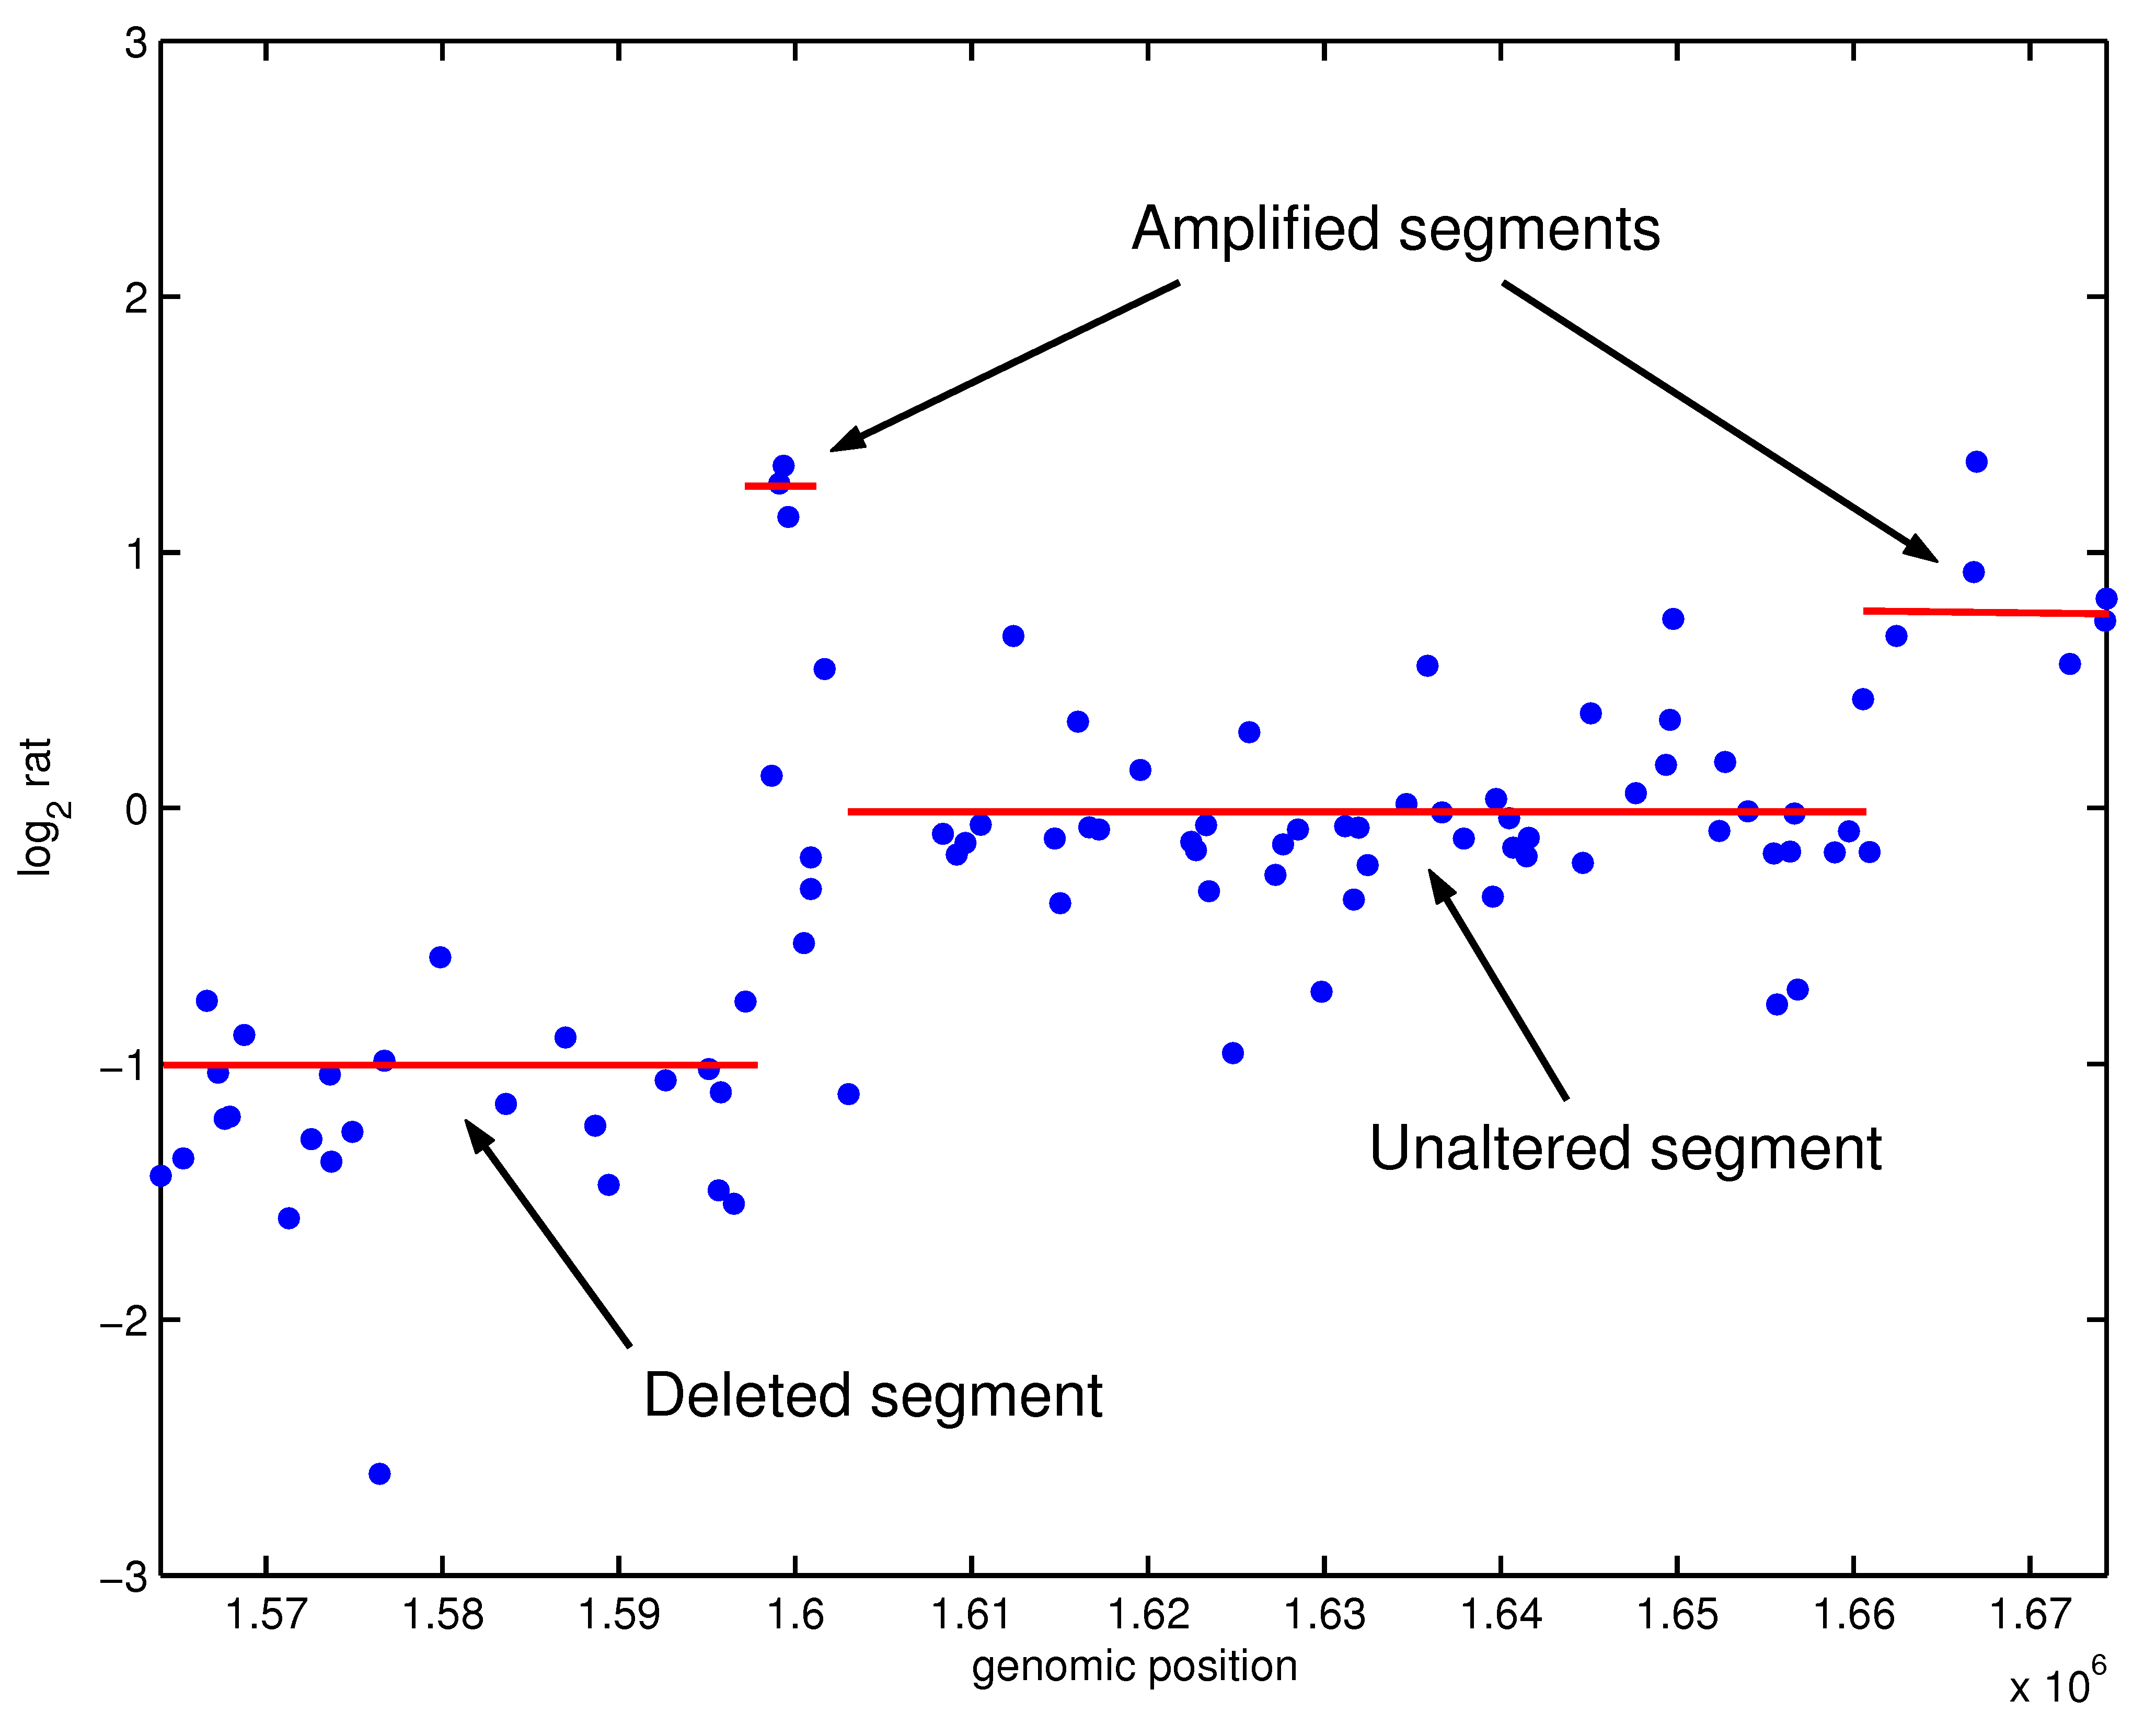
\epsfig{file = ../Figures/profile_example.eps, clip=,
%         width=.45\textwidth, height=.5\textheight}  \pause
      \epsfig{file = ../Figures/RigaillSoutenance.ps, clip=,
        width=.5\textwidth, height=.5\textheight}  \pause
    \end{tabular}
    &
    \hspace{-1cm}
    \begin{tabular}{p{.5\textwidth}}
      \paragraph{Issues:}
      \begin{itemize}
      \item \emphase{Algorithmics:} can not explore the segmentation
        space in a naive way,
      \item \emphase{'Confidence bounds'} for the breakpoint
        localisation $\tau_k$,
      \item \emphase{Model selection} to choose the number of
        breakpoints $K$.
      \end{itemize}
    \end{tabular}
  \end{tabular}
  }

%--------------------------------------------------------------------
%--------------------------------------------------------------------
\section{Single profile}
\subsection{Algorithmics}
%--------------------------------------------------------------------
\frame{\frametitle{Single profile: Algorithmics}

  \begin{itemize}
  \item Finding the optimal breakpoint localisation can be viewed as a
    \emphase{shortest path problem} 
  \item That can be solve via \emphase{dynamic programming} (DP) (see
    \refer{PRL05} for CGH)
  \item But with \emphase{quadratic complexity}: $O(Kn^2)$.
  \end{itemize} \pause

  \bigskip
  \begin{tabular}{cc}
    \hspace{-0.5cm}
    \begin{tabular}{p{.5\textwidth}}
      \begin{itemize}
      \item \emphase{'Pruned DP'} can strongly reduce the
        computational burden (\refer{Rig10}).
      \item Its theoretical worst complexity is the same as regular
        DP.
      \item Its mean empirical complexity is almost
        \emphase{linear}.
      \end{itemize} \\
      ~\\
    \end{tabular}
    &
    \hspace{-.5cm}
    \begin{tabular}{p{.5\textwidth}}
    \epsfig{file = ../Figures/Rig10-Fig.ps, clip=, bbllx=290,
      bblly=20, bburx=560, bbury=270, width=.4\textwidth}     
    \end{tabular}
  \end{tabular}

}

%--------------------------------------------------------------------
\subsection{Confidence bounds}
%--------------------------------------------------------------------
\frame{\frametitle{Single profile: Confidence bounds}
  %\vspace{-0.5cm}
  \begin{tabular}{cc}
    \hspace{-0.5cm}
    \begin{tabular}{p{.5\textwidth}}
      \begin{itemize}
      \item In a \emphase{Bayesian framework}, under factorisability
        assumptions (heteroscedastic model),  \\~
      \item all segmentations can be explored with
        complexity $O(Kn^2)$. \\~
      \item This allows to compute \emphase{exactly} quantities such
        as
        $$
        \Pr\{\tau_k \text{ is at position } t | \Ybf\}.
        $$
        \refer{RLR09}
      \end{itemize} 
      ~\\
      ~\\
    \end{tabular}
    &
    \hspace{-1cm}
    \begin{tabular}{p{.5\textwidth}}
      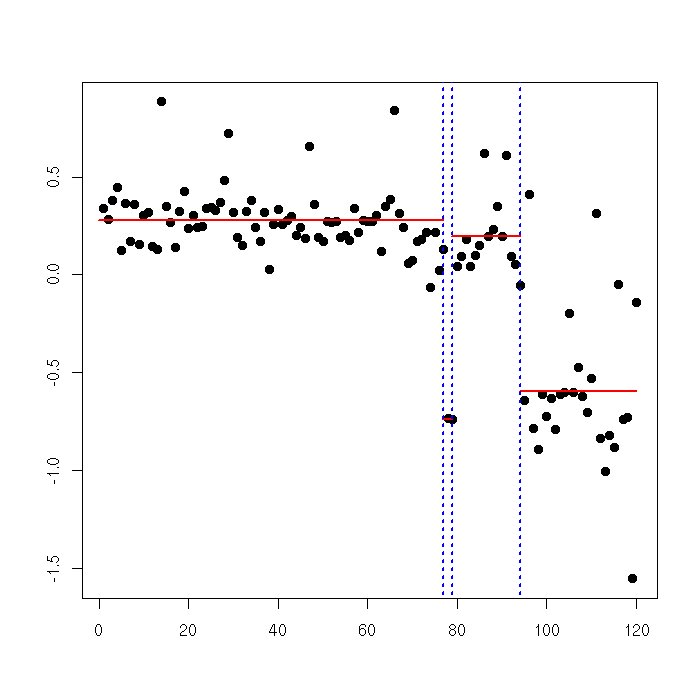
\includegraphics[width=0.45\textwidth, height=0.3\textheight,
      clip=]{\fighd/CopyNumberChr10_ICL}  \pause \\
      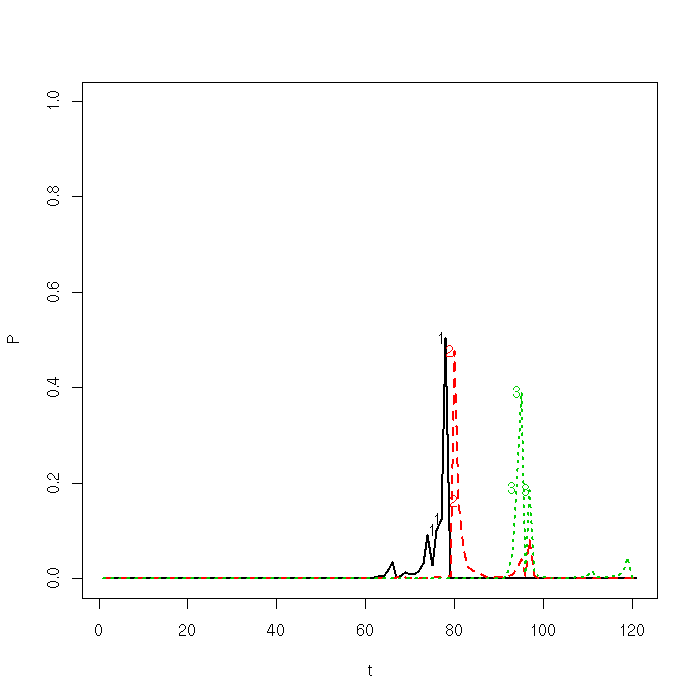
\includegraphics[width=0.45\textwidth, height=0.3\textheight,
      clip=]{\fighd/CopyNumberChr10_ProbaICL}  \pause \\
      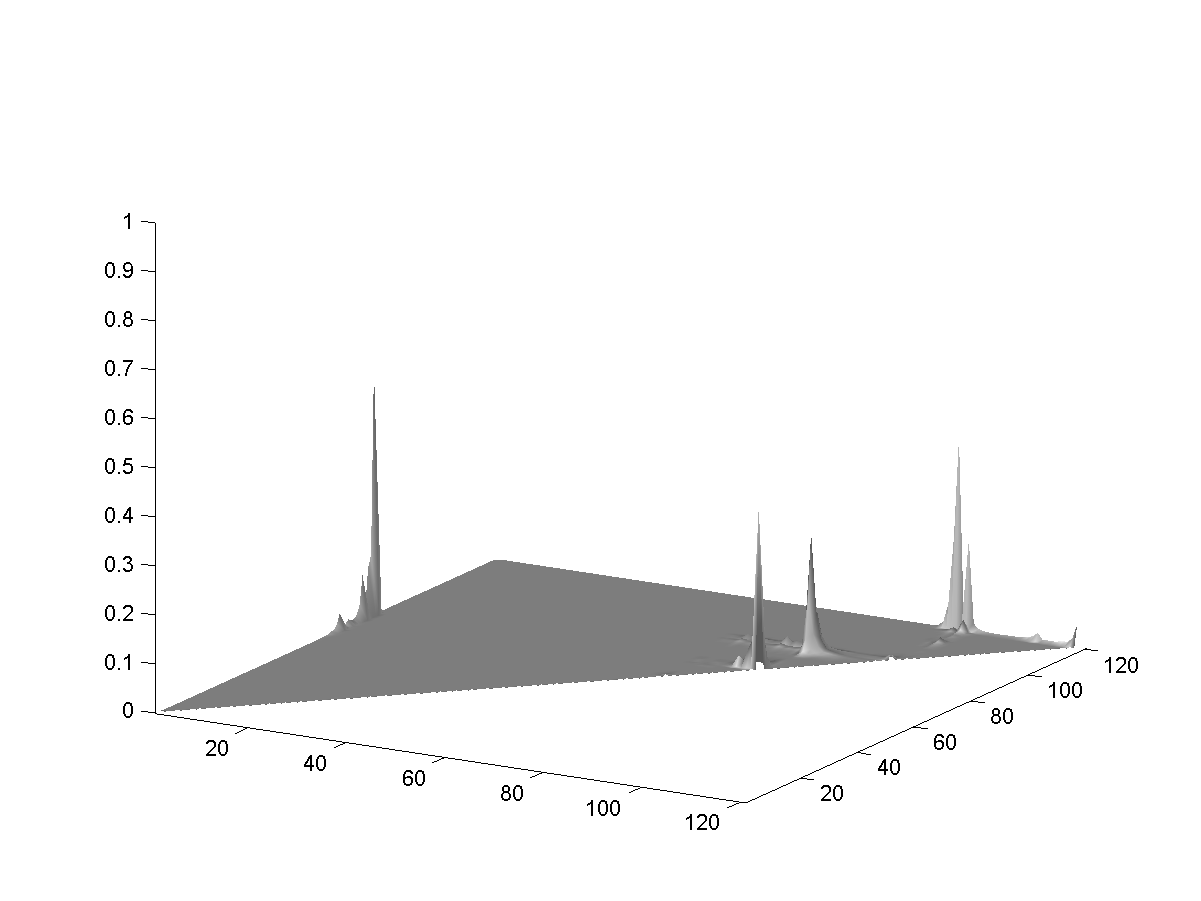
\includegraphics[width=0.45\textwidth, height=0.27\textheight,
      clip=]{\fighd/ProbSeg-ICL}   

    \end{tabular}
  \end{tabular}  
  }

%--------------------------------------------------------------------
\subsection{Model selection}
%--------------------------------------------------------------------
\frame{\frametitle{Single profile: Model selection}

%   Due to the discrete nature of the breakpoint positions, the
%   estimation (`'choice') of the number of segments $K$ is non trivial.

%   \bigskip
  \paragraph{Penalized contrast:} \refer{Leb05}
  $$
  \widehat{K} = \arg\min_K J_K + \frac{K}n \left(c_1 + \log \frac{n}K
    + c_2 \right), 
  \qquad 
  J_K = \sum_{k=1}^K \sum_{t \in I_k} (Y_t - \mu_k)^2.   \pause
  $$
  

  \paragraph{Asymptotic approximation:} \refer{ZhS07}
  $$
  \widehat{K} = \arg\max_K BIC(K), 
  \qquad
  BIC(K) \approx \log \left[ P(K|\Ybf) / P(0|\Ybf) \right].   \pause
  $$

  \paragraph{Exact calculation:} \refer{RLR09}
  $\begin{array}{rclcl}
    \widehat{K} & = & \displaystyle{\arg\max_K \log P(K|\Ybf)}, & &
    \text{similar  to } BIC(K) \\   
    \widehat{K} & = & \displaystyle{\arg\max_K \log P(K|\Ybf) - \Hcal(K)}, & &
    \Hcal(K) = \text{ entropy } \rightarrow ICL(K) \\   
    \widehat{m} & = & \displaystyle{\arg\max_m \log P(m|\Ybf)}, & & m = (t_k): 
    \text{ segmentation} 
  \end{array}$

  }

%--------------------------------------------------------------------
%--------------------------------------------------------------------
\section{Some extensions}
\subsection{Calling}
%--------------------------------------------------------------------
\frame{\frametitle{Extensions: Calling}

  \vspace{-0.5cm}
  \begin{tabular}{cc}
    \hspace{-0.5cm}
    \begin{tabular}{p{.5\textwidth}}
      \paragraph{Aim:} Assign a status (e.g. loss, gain) to each
      segment. \pause
      
      \bigskip
      \paragraph{Mixture model:} Each segment $I_k$ has an
      \emphase{unknown label $Z_k \in \{1, \dots P\}$}:
      \begin{eqnarray*}
        \Pr\{Z_k = p\} & = & \emphase{\pi_p} \\
        Z_k = p & \Rightarrow & \mu_k = \emphase{m_p}
      \end{eqnarray*} \pause

      \paragraph{Inference:} the EM algorithm can be combined with DP \\
      ~\\
      \ra 'DP-EM': \refer{PRL07} \\
      \ra R package \emphase{SegClust}
    \end{tabular}
    &
    \hspace{-.5cm}
    \begin{tabular}{p{.5\textwidth}}
      \epsfig{file = ../Figures/bt474_c1_seg_hetero_K2.eps, clip=,
        width=.45\textwidth, height=.35\textheight} \pause \\ 
      \\
      ~\epsfig{file = ../Figures/resultat_P3K8.eps , clip=,
        width=.45\textwidth, height=.35\textheight}  
    \end{tabular}
  \end{tabular}
  }

%--------------------------------------------------------------------
\subsection{Multiple profiles}
\frame{\frametitle{Extensions: Multiple profiles}
%--------------------------------------------------------------------
  \begin{tabular}{cc}
    \begin{tabular}{p{6cm}}
      Cancer studies often involve CGH profiles of numerous
      patients ($q \approx 100$). \\
      \bigskip
      Even when having the same disease, patients generally
      \emphase{do not have common breakpoints}.\\
      \bigskip
      Simultaneous analysis of all profiles $\{Y_{it}\}$ allows
      to \emphase{correct for artifacts} such as probe effect.\\
        \bigskip
      \refer{PLB11}
    \end{tabular}    
    &
    \begin{tabular}{p{6cm}}
      \hspace{-.75cm}
      \epsfig{file = ../Figures/nakao-mat.txt-MixSeg-V2.eps, bbllx=90,
      bblly=220, bburx=380, bbury=590, clip=, scale=.5}
    \end{tabular}
  \end{tabular}
  }

%--------------------------------------------------------------------
\frame{ \frametitle{Multiple array analysis}
  \paragraph{Simultaneous analysis of several profiles} allows us
  to 
  \begin{itemize}
  \item correct \emphase{technical biases}
  \item account for \emphase{covariates} associated with each sample
  \end{itemize} \pause 
  
  \bigskip
  \paragraph{Linear model framework:} \Refer{{\sl Picard} et al (2011a,
    2011b)}\nocite{PLB11}, \nocite{PLH11}  
  
  \medskip
  \begin{tabular}{p{.2\textwidth}p{.35\textwidth}p{.35\textwidth}}
%     \emphase{Task} & \emphase{Representation} & \emphase{Model} \\   
%     \hline
%     \\
    \emphase{Segmentation} & regression on unknown $\Tbf$: &
    $\displaystyle{\Ybf = \Tbf \mubf + \Ebf}$ \pause \\ 
    \\
    \emphase{\sl Correlation} & {\sl random probe effect: $\Ubf$}  &
    $\displaystyle{\sl \Ybf = \Tbf \mubf + \Zbf \Ubf + \Ebf}$  \\ 
    \\
    \emphase{Correction} & fixed covariates effect: $\theta$ &
    $\displaystyle{\Ybf = \Tbf \mubf + \Xbf \betabf + \Ebf}$ \pause \\  
    \\
    \emphase{Calling} & crosstabulation table $\Cbf$: &
    $\displaystyle{\Ybf = \Tbf \Cbf \mbf + \Ebf}$ \pause \\
    \\
    \emphase{Combinations} 
    & fixed + random effects: &
    $\displaystyle{\Ybf = \Tbf \mubf + \Xbf \betabf + \Zbf \Ubf + \Ebf}$ \\
    & fixed effects + calling: &
    $\displaystyle{\Ybf = \Tbf \Cbf \mbf + \Xbf \betabf + \Ebf}$  \\
  \end{tabular}
  }

%--------------------------------------------------------------------
\frame{\frametitle{CGHseg package}

  \textcolor{red}{Segmentation}+\textcolor{green}{calling}+
  \textcolor{blue}{fixed effects}:   
  $
  \Ybf = \textcolor{red}{\Tbf} \textcolor{green}{\Cbf} \mbf +
  \Xbf \textcolor{blue}{\betabf} + \Ebf
  $ 
  \epsfig{file = ../Figures/PLH11-V1-Fig1.eps, clip=, angle=270,
    bbllx=10, bblly=0, bburx=300, bbury=840, scale=0.4}        

  \bigskip
  \begin{itemize}
  \item \emphase{Correction:} functional versions (spline, wavelets)
    for the probe effect.
  \item \emphase{Presentation} at
    \url{www.agrocampus-ouest.fr/math/useR-2009/}
  \item \emphase{Soon on} \url{cran.r-project.org/}
  \end{itemize}

  }

%--------------------------------------------------------------------
\frame{\frametitle{Some simulations}

  \vspace{-0.5cm}
  \begin{tabular}{cc}
    \hspace{-0.5cm}
    \begin{tabular}{p{.5\textwidth}}
      Correction and calling improve
      \begin{itemize}
      \item estimation of $K$, 
      \item breakpoint detection (FDR / FNR), 
      \item true signal recovery.
      \end{itemize}
      
      \bigskip
      \paragraph{Calling:} yes = --, no = - -

      \bigskip
      \paragraph{Correction:} \\
      $\blacksquare =$ no correction, \\
      \textcolor{red}{$\bullet = $ position  specific}, \\
      \textcolor{blue}{$\triangle =$ spline}, \\
      \textcolor{green}{$\diamond =$ wavelet}, \\
      \textcolor{orange}{$\circ =$ CBS} 
    \end{tabular}
    &
    \hspace{-1cm}
    \begin{tabular}{p{.5\textwidth}}
      \epsfig{file = ../Figures/PLH11-V1-Fig2.eps, clip=,
        width=.5\textwidth, height=0.85\textheight}        
    \end{tabular}
  \end{tabular}

  }

%--------------------------------------------------------------------
\subsection{Recurrent alterations}
%--------------------------------------------------------------------
\frame{\frametitle{Extensions: Recurrent alterations}
  
  \vspace{-0.5cm}
  \begin{tabular}{cc}
    \hspace{-.5cm} 
    \begin{tabular}{p{.2\textwidth}}
      \textcolor{red}{$\bullet $ gain} / \textcolor{blue}{$\bullet $ loss} \\
      \epsfig{file=../Figures/ExMinRegion.eps, width=0.2\textwidth,
        height=0.75\textheight, clip=, bbllx=270, bblly=209, bburx=400,
        bbury=593} 
    \end{tabular}
    &
    \hspace{-0.5cm}
    \begin{tabular}{p{.7\textwidth}}
      \paragraph{Aim:} Detect recurrent alterations among a set of
      profiles (patients). \pause

      \bigskip
      \paragraph{Example.} $M^* = 31$ patients present \emphase{$\ell =
      5$ successive deletions} between probes 1189 and 1193, in
      chromosome 9. 

      \bigskip
      \paragraph{Question.} Is this \emphase{significant}, given the
      number of patients ($m=84$) and the profiles length ($n=2340$)? 

      \bigskip \pause
      \paragraph{Upper bound.} The $p$-value is smaller than 
      $$
      \Pr\{\exists t : X_{-, t} \dots X_{-, t+\ell-1} > M^*\}, 
      $$
      which can be computed exactly (\Refer{R. \& Stefanov
        (2009)}\nocite{RoS09}). 
    \end{tabular}
  \end{tabular}

  }

%--------------------------------------------------------------------
%--------------------------------------------------------------------
\section{Conclusion}
\subsection{Alternative strategies}
%--------------------------------------------------------------------
\frame{\frametitle{Alternative strategies}

  \paragraph{Comparative studies (\refer{LJK05}, \refer{WiF05}):}
  segmentation turns out to be the most efficient approach for CGH
  analysis. \pause

  \bigskip\bigskip
  \paragraph{Hidden Markov Models (HMM):}
  \begin{itemize}
  \item Naturally provides segment calling
  \item With implicit assumption on the distribution of the segment
    lengths,
  \item But may allow flexible modelling. \pause
  \end{itemize}

  \bigskip\bigskip
  \paragraph{Functional analysis}
  \begin{itemize}
  \item Allows flexible (but smooth) correction functions,
  \item Can also perform segmentation (using relevant wavelet basis). 
  \end{itemize}
  }

%--------------------------------------------------------------------
\subsection{Perspectives and comments}
%--------------------------------------------------------------------
\frame{\frametitle{Perspectives and comments}

  \paragraph{On-going work}
  \begin{itemize}
  \item Segmentation of correlated profiles with arbitrary correlation
    structure,
  \item Fast ('pruned DP') segmentation/calling algorithm,
  \item Extension to NGS (large and discrete signal + overlapping
    reads). \pause
  \end{itemize}

  \bigskip\bigskip
  \paragraph{As for the CNV-maize:} Segmentation techniques strongly
  rely on the 
  \begin{itemize}
  \item knowledge of the \emphase{probe positions}
  \item along a \emphase{reference genome}
  \end{itemize}
  }

%--------------------------------------------------------------------
\subsection{Appendix}
%--------------------------------------------------------------------
{\tiny
  \bibliography{/Biblio/ARC,/Biblio/AST,/Biblio/SSB}
  \bibliographystyle{/Latex/astats}
  %\bibliographystyle{plain}
  }

%--------------------------------------------------------------------
\frame{ \frametitle{Appendix: A CGH profile: $K = 3, 4$}
  \vspace{-.25cm}
  \begin{tabular}{lll}
    \hspace{-0.5cm}
    \begin{tabular}{p{0.2\textwidth}} Optimal segmentation \end{tabular}
    &
    \hspace{-0.5cm}
    \begin{tabular}{c}
      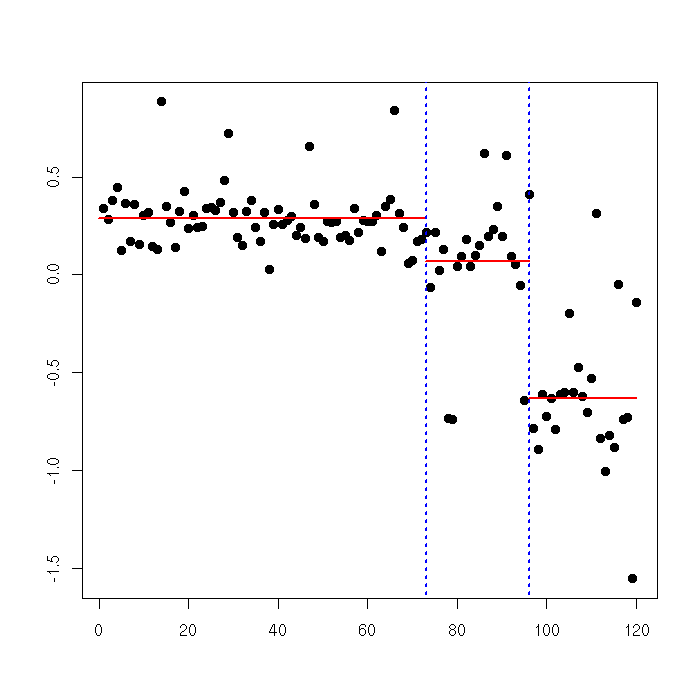
\includegraphics[width=0.35\textwidth, height=0.3\textheight,
      clip=]{\fighd/CopyNumberChr10_BIC}   
    \end{tabular}
    &
    \hspace{-0.5cm}
    \begin{tabular}{c}
      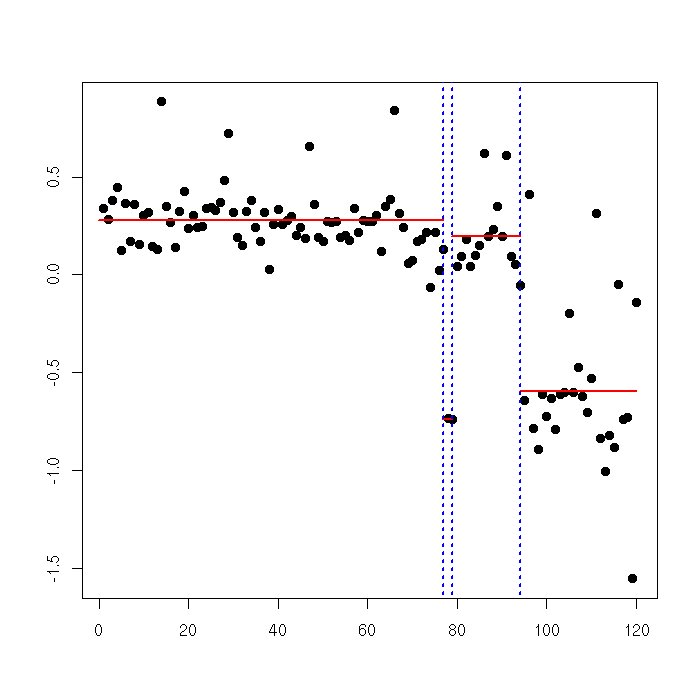
\includegraphics[width=0.35\textwidth, height=0.3\textheight,
      clip=]{\fighd/CopyNumberChr10_ICL}  
    \end{tabular} \\ 
    \hspace{-0.5cm}
    \begin{tabular}{p{0.2\textwidth}} Breakpoint position \end{tabular}
    &
    \hspace{-0.5cm}
    \begin{tabular}{c}
      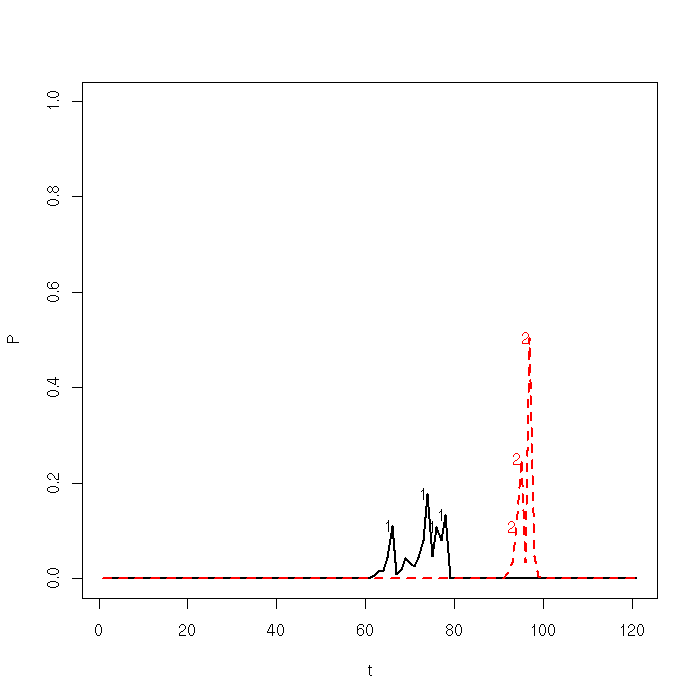
\includegraphics[width=0.35\textwidth, height=0.3\textheight,
      clip=]{\fighd/CopyNumberChr10_ProbaBIC}  
    \end{tabular}
    &
    \hspace{-0.5cm}
    \begin{tabular}{c}
      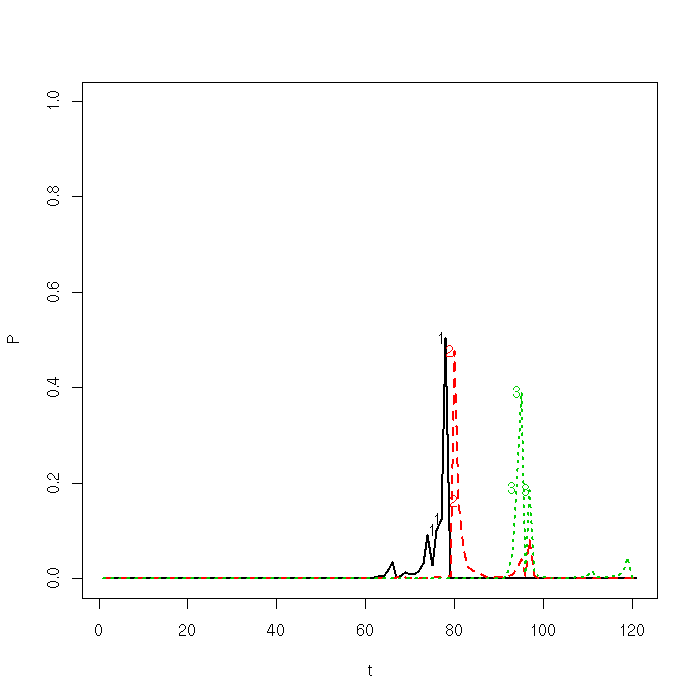
\includegraphics[width=0.35\textwidth, height=0.3\textheight,
      clip=]{\fighd/CopyNumberChr10_ProbaICL}  
    \end{tabular} \\ 
    \hspace{-0.5cm}
    \begin{tabular}{p{0.2\textwidth}} Segment probability \end{tabular}
    &
    \hspace{-0.5cm}
    \begin{tabular}{c}
      \vspace{-.5cm}
      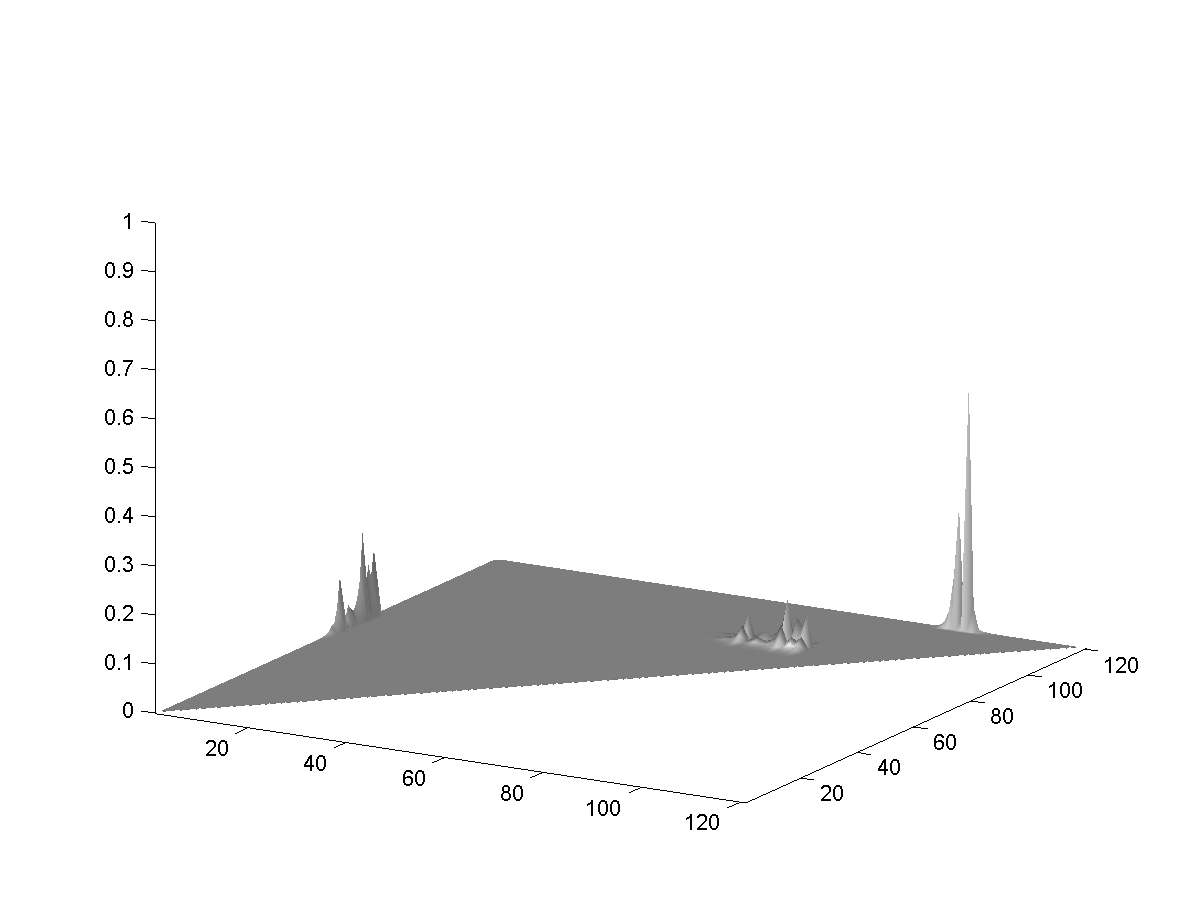
\includegraphics[width=0.35\textwidth, height=0.35\textheight,
      clip=]{\fighd/ProbSeg-BIC}     
    \end{tabular}
    &
    \vspace{-.5cm}
    \begin{tabular}{c}
      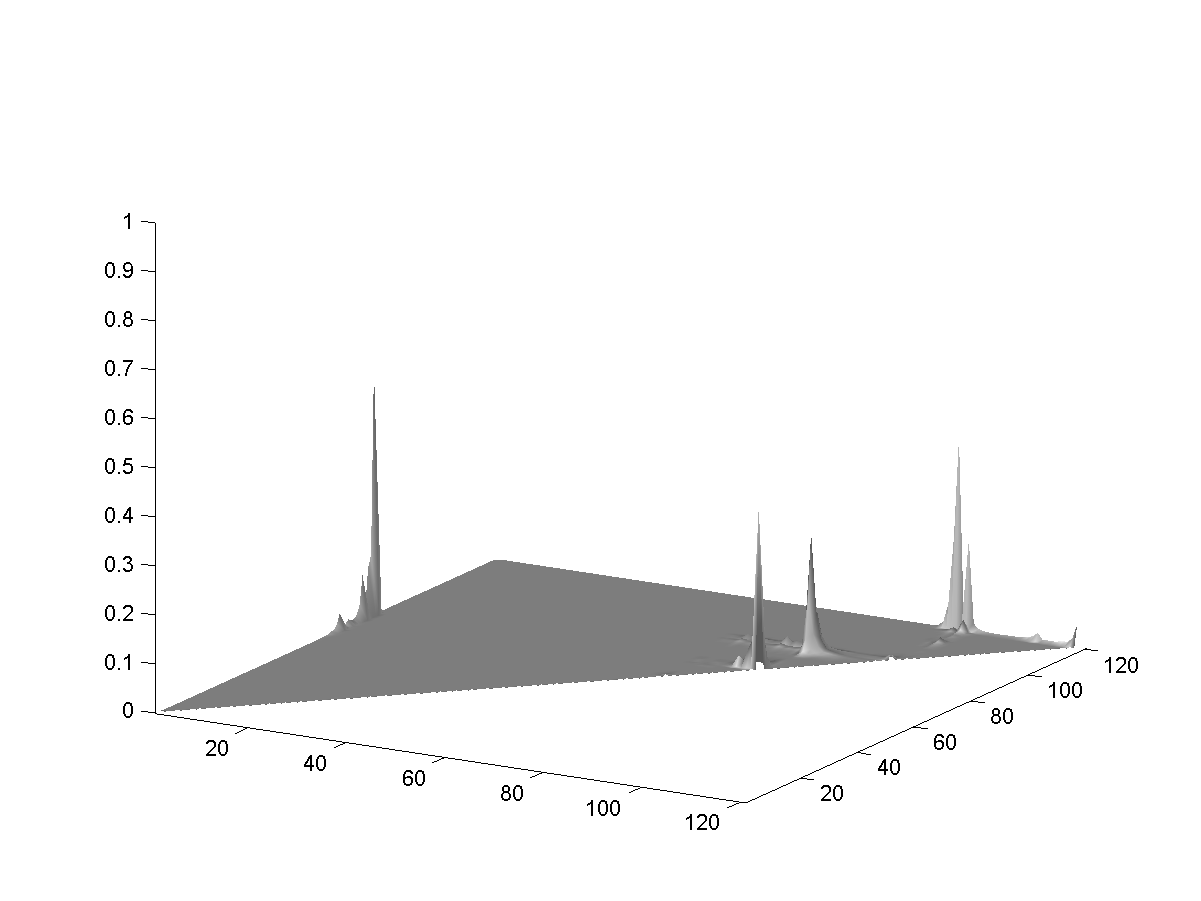
\includegraphics[width=0.32\textwidth, height=0.27\textheight,
      clip=]{\fighd/ProbSeg-ICL}   
    \end{tabular} 
  \end{tabular}
  }

%--------------------------------------------------------------------
%--------------------------------------------------------------------
\end{document}
%--------------------------------------------------------------------
%--------------------------------------------------------------------

\frame{\frametitle{}
  }

  \vspace{-0.5cm}
  \begin{tabular}{cc}
    \hspace{-0.5cm}
    \begin{tabular}{p{.5\textwidth}}
    \end{tabular}
    &
    \hspace{-1cm}
    \begin{tabular}{p{.5\textwidth}}
    \end{tabular}
  \end{tabular}
